\chapter{Materials and Methods}

In order to successfully identify and design benzylisoquinoline alkaloid-based drug leads targeting PTP1B and IKK-$\beta$ complexes as treatments for PCOS insulin resistance, the study will follow the methodology summarized in \ref{fig:methodology}. The software and databases involved include BIadb database, MTiOpen Screen web server, AutoDock Tools, GROMACS, PubChem, MarvinSketch, PocketDB and PrankWeb, AutoDock Vina, Open 3D-Align, Open 3D-QSAR, LigPlot, SwissADME, ProToxII, PSC-db, and Super Natural 3.0. Molecular docking of the 30 derivatized ligands with human  PTP1B and IKK-$\beta$ complexes will be performed. Based on the subsequent chemometric analysis, modifications will be made to the ligands to further optimize their interactions. Afterward, the most potent modified ligand exhibiting the relatively best interactions with human IKK-$\beta$ and PTP1B will undergo an online database search, focusing on identifying natural plant sources with molecules possessing similar structures. 

\begin{figure} 
            \centering
            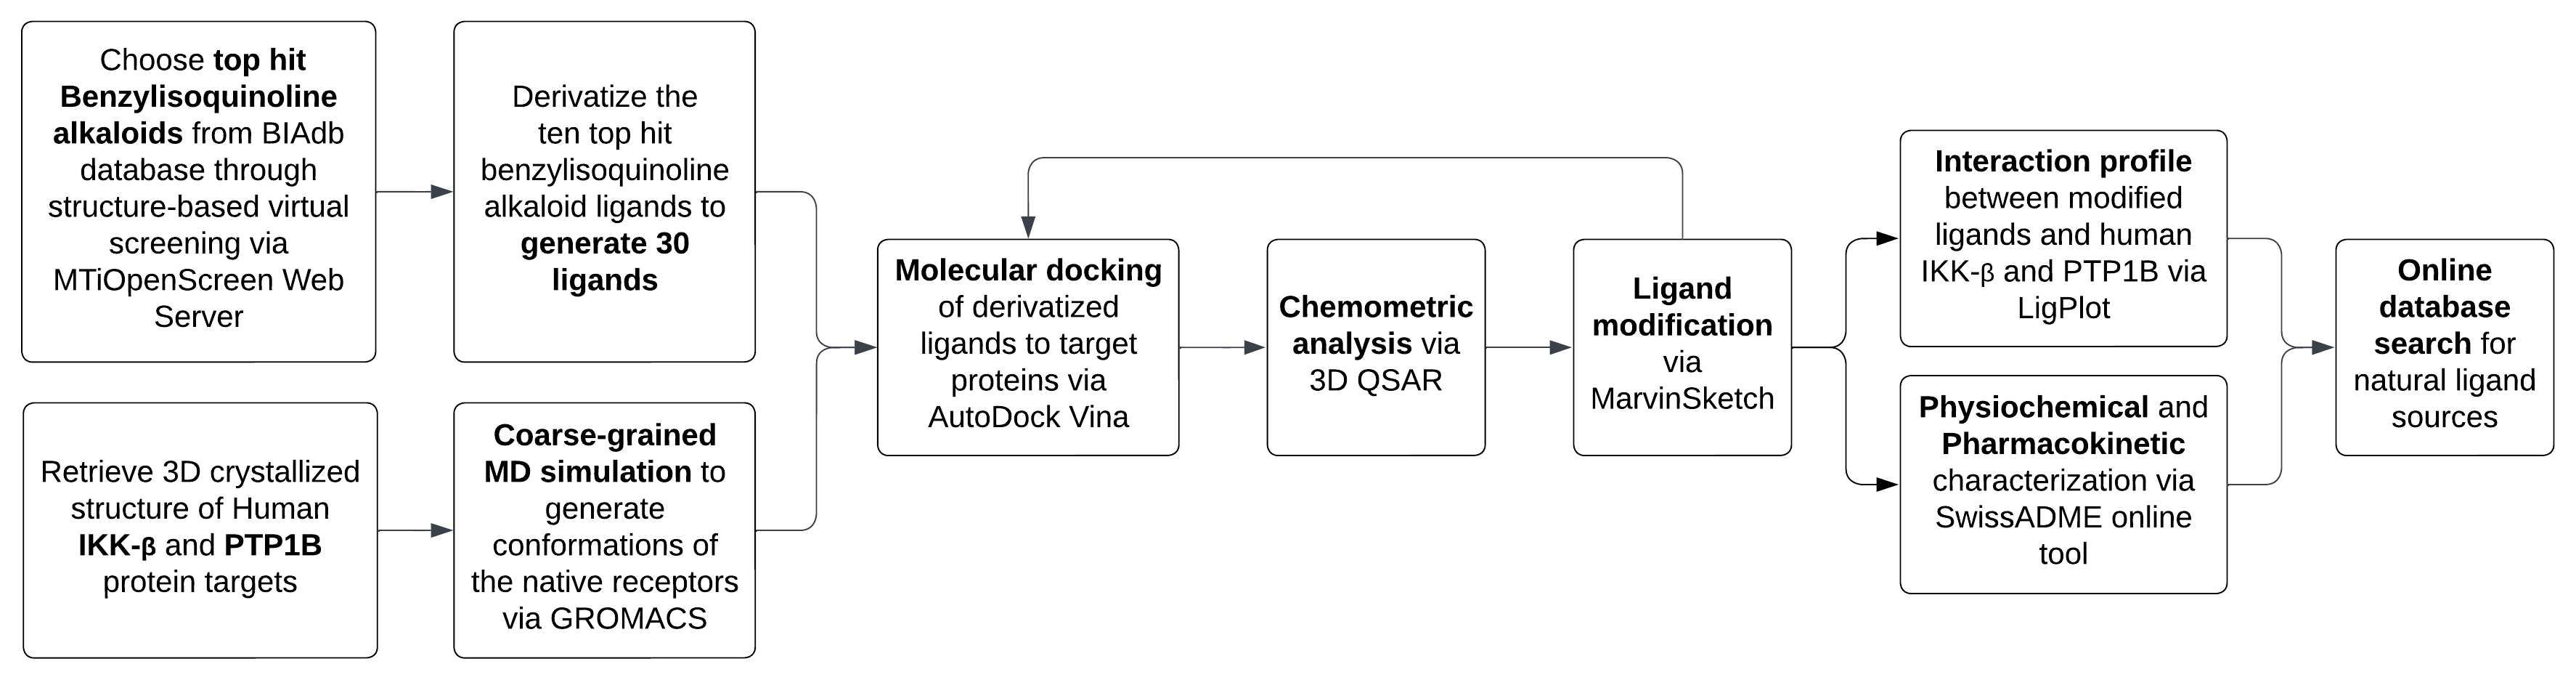
\includegraphics[width=1\linewidth]{Images/Flowchart of Methods.png}
            \caption{Overview of methodology}
            \label{fig:methodology}
        \end{figure}


\section{Initial Ligand Data Set}
Benzylisoquinoline alkaloids targeted for human IKK-$\beta$ and PTP1B  will be filtered and chosen based on lead-likeness (i.e., 250$<$MW$<$350 Da and -4$<$XlogP$<$3.5) and backbone similarity to berberine from the BIadb database. A structure-based virtual screening of the selected benzylisoquinoline alkaloids will be conducted using MTiOpenScreen web server to identify the top 10 ligands against the prepared human IKK-$\beta$ and PTP1B targets.  Each of the ten top hit benzylisoquinoline alkaloid ligands selected from the structure-based virtual screening will be derivatized to obtain 30 ligands for ensemble docking and 3D QSAR analysis. 

\section{Receptor and Ligand Preparation}
The three-dimensional (3D) crystallized structure of human IKK-$\beta$ (PDB ID: \href{https://www.rcsb.org/structure/4KIK}{4KIK}) and PTP1B (PDB ID: \href{https://www.rcsb.org/structure/4I8N}{4I8N}) will be retrieved from the Protein Data Bank, an open access database with 3D protein conformations. Each wild-type receptor will be prepared for subsequent protocols by removing ligand and solvent molecules and adding hydrogen atoms via AutoDock Tools. 

\subsection{Coarse-grained Molecular Dynamics Simulation}
The initial system will be minimized in a vacuum and equilibrated using GROMACS, an open-source software primarily used for biomolecule dynamical simulations. A coarse-grained molecular dynamic (MD) simulation will be run to generate conformations of the native receptors for subsequent ensemble docking. 

Preprocessing of the protein systems will be done by removing heteroatoms. The secondary structures of IKK-$\beta$ and PTP1B will be found and the All-atom models of the systems will be martinized and converted to Coarse grain models using the Martinize python script. As a result, the coarse-grained structures, corresponding topology, and parameter files for the proteins will be generated. Moving on to system preparation for MD simulation, the 'insane' tool to build coarse-grain systems via the 'insane.py' script will be employed to facilitate the solvation and ion addition (i.e., $Na^+$ or $Cl^-$) for system neutrality. 

The Martini 3 force field will be used to unite groups of atoms into effective interaction sites (Paulo et al., 2020). The topology file will be modified to include the parameters required for simulation, incorporating it with the Martini 3 force field. Once the solvated system has been prepared, standard molecular dynamics (MD) simulation protocols will be employed. The energy of the system will be minimized and followed by equilibration. Afterward, a production run of 2$\mu$s will be performed. From the trajectory, an ensemble of PDB files will be extracted via the 'trajout' command wherein the first 10 frames of the trajectory will be included in the file. The resulting pdb file will contain the native conformations of the systems and can initially be visualized using UCSF Chimera.

\section{Ensemble Docking}
The 3D structures of the benzylisoquinoline alkaloid derivatives from 3.0.1 will be obtained from the PubChem Database. Derivatives of the top ten hits will be created and prepared using MarvinSketch. Their geometries will be optimized in Avogadro using the GAFF force field. Afterward, the prepare$_$ligand tool in MGLTools will be used to prepare the compounds for molecular docking to the IKK-$\beta$ and PTP1B ensembles. 

To execute targeted docking, grid box coordinates will be set based on the binding sites of native ligands as predicted by PocketDB and PrankWeb as well as assessments of existing crystal structures. A grid box of 40x40x40 (xyz) and with a 0.375 \r{A} spacing will be used to fully encapsulate the binding sites. AutoDock Vina will be used to predict the ligand-protein interactions. The output is the calculated binding energies and poses for each ligand-target complex based on van der Waals, electrostatic, and hydrogen-bond potentials derived from AMBER force fields. 

\section{3D-QSAR Analysis}
The best resulting pose for each ligand from the molecular docking step will be subjected to chemometric analysis using Open 3D-Align and Open 3D-QSAR. First, Open3D-Align will be used to import the 3D molecular structures of benzylisoquinoline alkaloid ligands and will subsequently be best-aligned. Open 3D-QSAR will then be used to determine the areas favoring or disfavoring functional groups (i.e., steric, electronegative, and electropositive groups) based on non-covalent interactions between the ligand and IKK-$\beta$ and PTP1B respectively. Molecular interaction fields will be computed using AMBER FF99 Van der Waals parameters (steric fields) and a point charge model (electrostatic field). The dataset will be split into training and test sets for later external validation. 

Pretreatment operations will be executed to exclude poorly informative variables that may affect the validity of the model. The following parameters will be met: (1) a grid box with 1.0 \r{A} step size and 5.0 \r{A} outgap; (2) 1.0 x 10$^4$ kcal/mol steric cutoff; (3) 30.0 kcal/mol energy cutoff; zeroing of low energy values ($<$0.05 kcal/mol); (4) exclusion of N-level variables and variables with low standard deviations ($<$0.1); and blocking of unweighted scaling. 

A partial least squares (PLS) model will be built to identify and extract the quantitative influence of specific chemical features of molecules on their biological activity. Cross-validation will be carried out to challenge the internal predictivity of the model (LOO, LTO, LMO). External prediction against the test set will also be used to assess the predictive ability of the model. Moreover, the predictivity may also be improved using fractional factorial design (FFD) variable selection. 

The model's internal and external predictive capability will be validated using the output of cross-validation methods and non-cross-validation methods where q$^2$$>$0.5, r$^2$$>$0.6, and r$^2$pred$>$0.6 with the lowest standard estimation error (SEE). 

The 3D-QSAR model will be visualized with PyMOL. Contour plots representing sterically favored, sterically disfavored, electronegative, and electropositive regions will be used as supporting guides for ligand functionalization. 

\section{Ligand Optimization}
The benzylisoquinoline alkaloid ligands will be modified in MarvinSketch using the results obtained from the 3D-QSAR model. Ligands that demonstrated the highest binding affinities will be used as model ligands when adding substituents. The functionalized compounds will be redocked using the same parameters as in the previous docking step to determine if the structural changes on ligands improved binding affinities to each target receptor.

\section{Protein-ligand interaction analysis}
The interaction profile between the modified benzylisoquinoline alkaloid ligands and human IKK-$\beta$ and PTP1B (e.g. hydrophobic interactions and hydrogen bonds) will be determined by using LigPlot. The presence and strength of intermolecular interactions will be obtained from the generated 2-D schematic representation of the protein-ligand complexes. 

\section{ADME and Toxicity Analysis}
The modified ligands will be subjected to the \href{http://www.swissadme.ch/}{SwissADME} online tool to determine and evaluate their predicted physicochemical and pharmacokinetic characteristics. Such data to be examined include physicochemical properties, lipophilicity, water-solubility, pharmacokinetics, drug-likeliness, and medicinal chemistry to investigate its bioavailability and therapeutic potential (Kumar et al., 2022). Furthermore, \href{https://tox-new.charite.de/protox_II/} {ProToxII} will be used to predict the modified ligands' toxicity in terms of LD50, hepatotoxicity, carcinogenicity, immunotoxicity, mutagenicity, and cytotoxicity. 

\section{Online database Search for natural ligand sources}
The top modified ligand that showed the highest binding affinity and optimal physicochemical and pharmacokinetic characteristics when bound to human IKK-β and PTP1B will be subjected to an online database search to determine if it can be naturally sourced from plants. Specifically, molecules that possess identical structures, which may be primary or secondary metabolites, will be searched. Databases such as the Plant Secondary Compounds Database (\href{https://www.ncbi.nlm.nih.gov/pmc/articles/PMC7924326/}{PSC-db}) and \href{https://www.ncbi.nlm.nih.gov/pmc/articles/PMC4384003/}{Super Natural 3.0} will be utilized.  
